\documentclass{X:/Documents/Coding/Latex/myassignment}
\title{Mathematical Biology Assignment 3 \& 4}

\begin{document}
\maketitle
Normally I would paraphrase the  the questions, but instead I have appended the question sheet to the end
\section{Assignment 3}
\begin{enumerate}
	\item to break down the problem into pieces:
	\begin{itemize}
		\item The cells $(c,m,n)$ all proliferate logistically ($c$ greater rate than $n$).
		\item $m$ increases (and saturates) with $a$
		\item $c,n,m$ all move by random motion, and $m$ moves via chemotaxis with gradient of $a$
		\item $a$ is produced constantly by $c$ and decays `naturally'
		\item $m$ kills $c$ at a rate proportional to $a$ concentration. 
		\item $a$ moves via diffusion
	\end{itemize}
	Constants:
	\begin{itemize}
		\item Proliferation rates of $c,m,n$ respectively $p_c,p_m,p_n$ with $p_c > p_n$
		\item Carrying capacities for the cells $k_c,k_m,k_n$
		\item 
	\end{itemize}
	\begin{align*}
		\dd ct\\
		\dd nt\\
		\dd mt\\
		\dd at\\
	\end{align*}
	\item 
	\begin{enumerate}
		\item Sub in the given solution form. I'm going to let $(\tilde{b}, \tilde{p}) = \epsilon(b_1,p_1)e^{iqx+\lambda t}$ 
		\begin{align*}
			\dd bt &= \mu \ddn bx2 + \frac{\gamma b}{1+ b} - \frac{b p }{\kappa + b}\\
			\lambda \tilde{b} &= -q^2 \mu \tilde{b} + \frac{\gamma \tilde{b}}{1 + \tilde{b}} - \frac{\tilde{b} (1 + \tilde{p})}{\kappa + b}\\
			\lambda &= -q^2 \mu + \frac{\gamma}{1 + \tilde{b}} - \frac{(1+\tilde{p})}{\kappa + \tilde{b}}\\
		\end{align*}
		To leading order, $(\tilde{b},\tilde{p})$ is negligible (assuming $\epsilon \ll 1$) this gives
		\[\lambda = -q^2 \mu + \gamma - \frac{p}{\kappa}\]
		For the $p$ equation:

		\begin{align*}
			\dd pt &= \ddn px2 - \delta \dd{}x \left(p \dd bx\right) + \alpha (1 + \sigma b -p)\\
			\dd pt &= \ddn px2 - \delta \left(\dd px \dd bx + p \ddn bx2\right) + \alpha (1 + \sigma b -p)\\
			\lambda \tilde{p} &= -q^2 \tilde{p} - \delta\left(-q ^2\tilde p \tilde b - (1+ \tilde{p})q^2 \tilde{b}\right)+ \alpha (1 + \sigma \tilde{b} - (1 + \tilde{p}))\\
			\lambda &= -q^2 - \delta\left(-q ^2\tilde b - q^2 \tilde{b}\right)+ \alpha (\sigma \frac{b_1}{p_1} - 1)\\
		\end{align*}

		%need to end up with
		%\[\lambda = -q^2 - \alpha\]
		\item Instabilities occur for lambda with positive real part. So, assuming real $q$, the most likely instabilities will occur for small $q$
		\item 
	\end{enumerate}
	\item 
	\begin{enumerate}
		\item The $\chi$ terms represent chemotaxis along a gradient. Since negative coefficients correspond to moving up a gradient (towards higher concentrations), $c_1$ is the $\beta$-amyloid, and $c_2$ is the TNF-$\alpha$.
		\item Sub in $(m_0,c_{10},c_{20})$. The first equation is trivially zero.
		% \begin{align*}
		% 	\dd mt &= D_m \ddn mx2 - \chi_1 \dd{}x \left(m \dd {c_1} x\right) + \chi_2 \dd{}x \left(m \dd{c_2}x\right)\\
		% \end{align*}
		\begin{align*}
			\dd{c_1} t &= D_1 \ddn{c_1}x2 + a_1 m - b_1 c_1\\
			0 &= 0 + a_1m_0 - b_1 c_{10}\\
			c_{10} &= \frac{a_1 m_0}{b_1}
		\end{align*}
		\begin{align*}
			\dd{c_2} t &= D_2 \ddn{c_2}x2 + a_2 m - b_2c_2\\
			0 &= 0 + a_2 m_0 - b_2 c_{20}\\
			c_{20} &= \frac{a_2 m_0}{b_2}
		\end{align*}
		\item $\epsilon_1 = \frac{D_m}{D_1}$. This is the ratio of the rates of diffusion of glial cells and $\beta$-amyloid. Similarly, $\epsilon_2$ is the ratio of the rates of diffusion of glial cells and TNF-$\alpha$.
		Setting these simultaneously to zero corresponds to $D_m \ll D_1,D_2$. I.e. that the rate of diffusion of glial cells is significantly lower than that of the protein and chemical. Explicitly setting these to zero is by either letting $D_m = 0$ or both $D_1,D_2 \to \infty$. I.e. by assuming glial cells do not diffuse or that the protein and chemical both diffuse instantly.
		\item 
		\item 
		\item 
	\end{enumerate}
\end{enumerate}

\clearpage
\section{Assignment 4}

\begin{enumerate}
	\item 
	\begin{enumerate}
		\item $u$ is an activator, and $v$ is an inhibitor, as $u$ promotes the growth of $u$ and $v$, while $v$ inhibits the growth of $u$.
		\item Spatially uniform steady state:
		\begin{align*}
			\frac{u^2}{v} - \beta u &= 0\\
			u^2 - v &= 0
		\end{align*}
		Setting $v = u^2$ gives $u = \frac{1}{\beta}$. I.e. there is a unique spatially uniform steady state for $u = \frac{1}{\beta}$ and $v = \frac{1}{\beta^2}$.
		\item
		\[(u,v) = (\frac{1}{\beta}, \frac{1}{\beta^2}) + \epsilon (u_1,v_1) e^{iqx + \lambda t} + \bigo(\epsilon^2)\] 
		Again ill let $(\tilde{u},\tilde{v}) = \epsilon (u_1,v_1) e^{iqx + \lambda t} $.

		This question is slightly poorly posed as the $\bigo(\epsilon^2)$ v term could interact with the $u^2$ $\bigo(\epsilon)$ term to give $\bigo(1)$...
		\begin{align*}
		\dd ut &= \frac{u^2}{v} - \beta u + \ddn ux2\\
		\end{align*}

		\begin{align*}
		\dd vt &= u^2 - v + \delta \ddn vx2\\
		\end{align*}
		\item 
		\item 
	\end{enumerate}
	\item 
	\begin{enumerate}
		\item 
		\item 
		\item 
		\item 
	\end{enumerate}
\end{enumerate}



% \section*{Code}
% \lstinputlisting{A3Code.m}

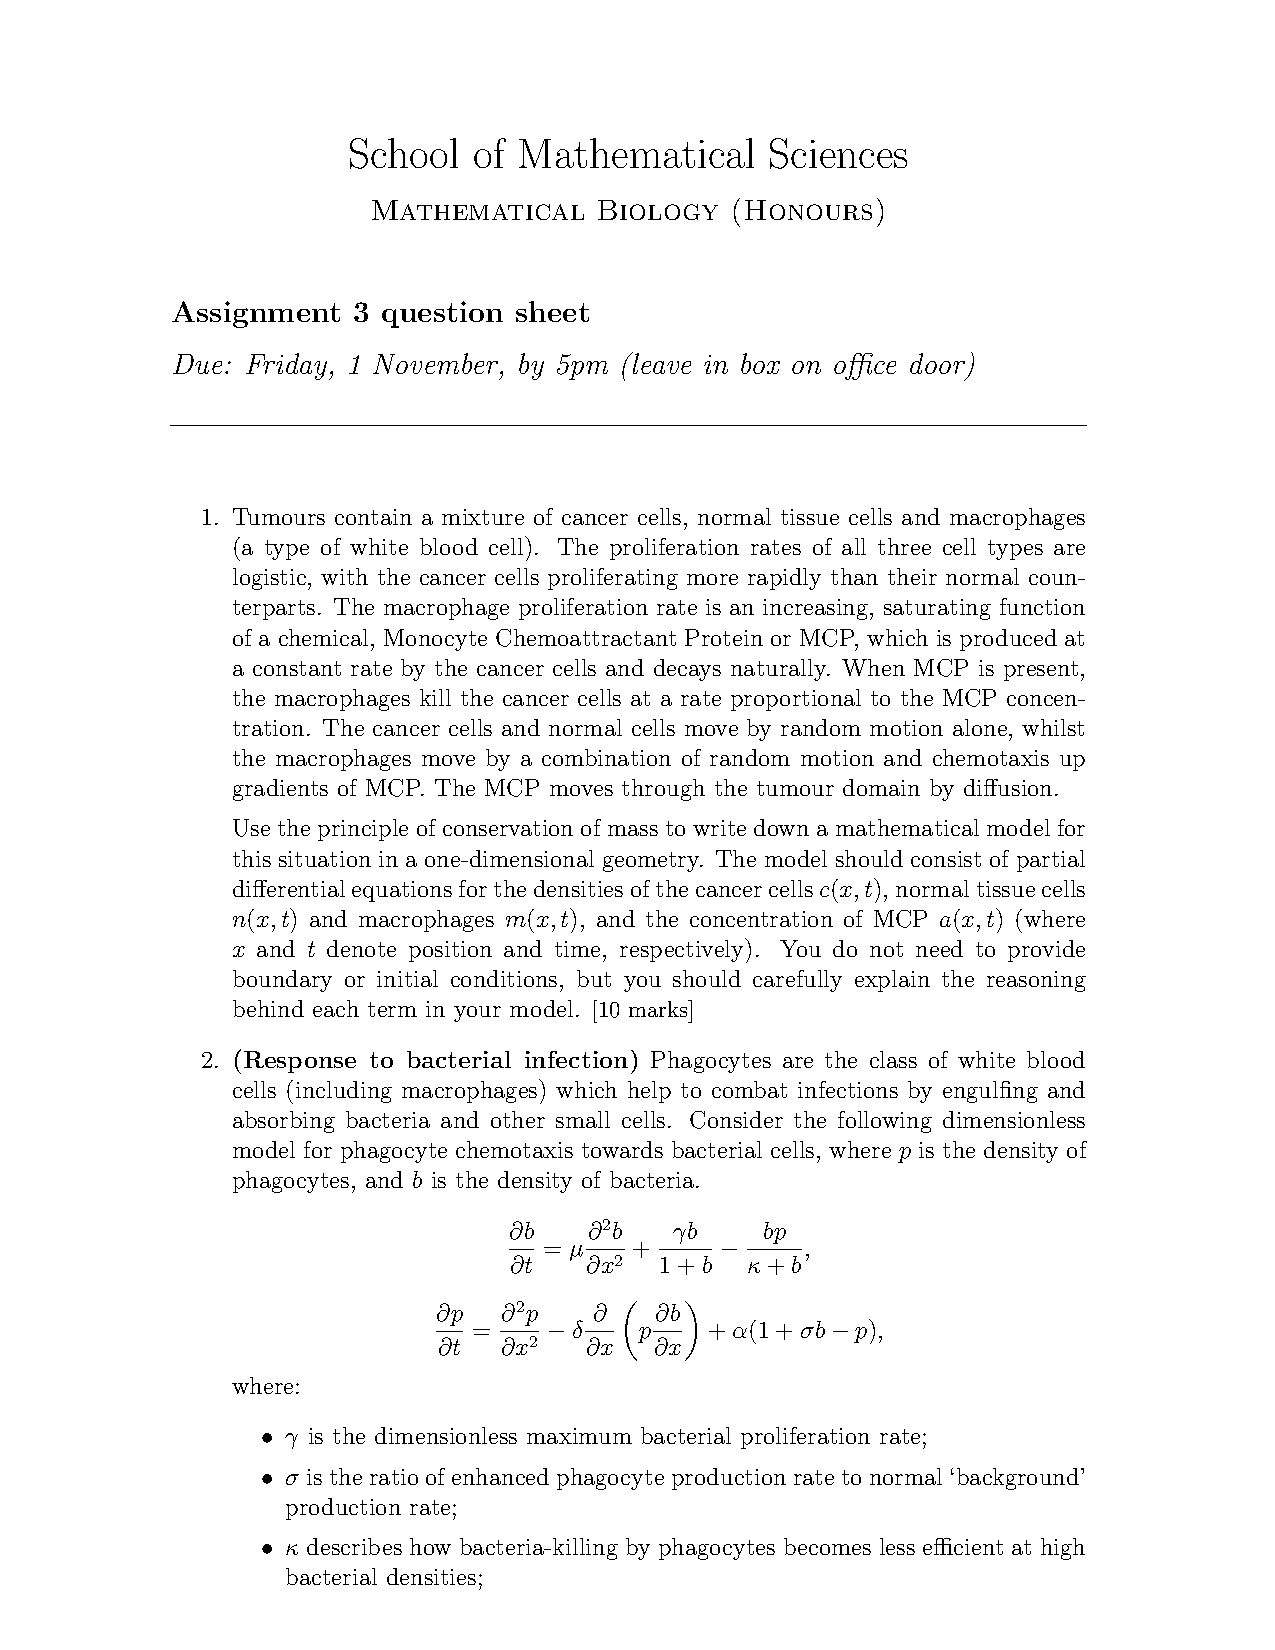
\includepdf[pages=1-]{A3_2019.pdf}
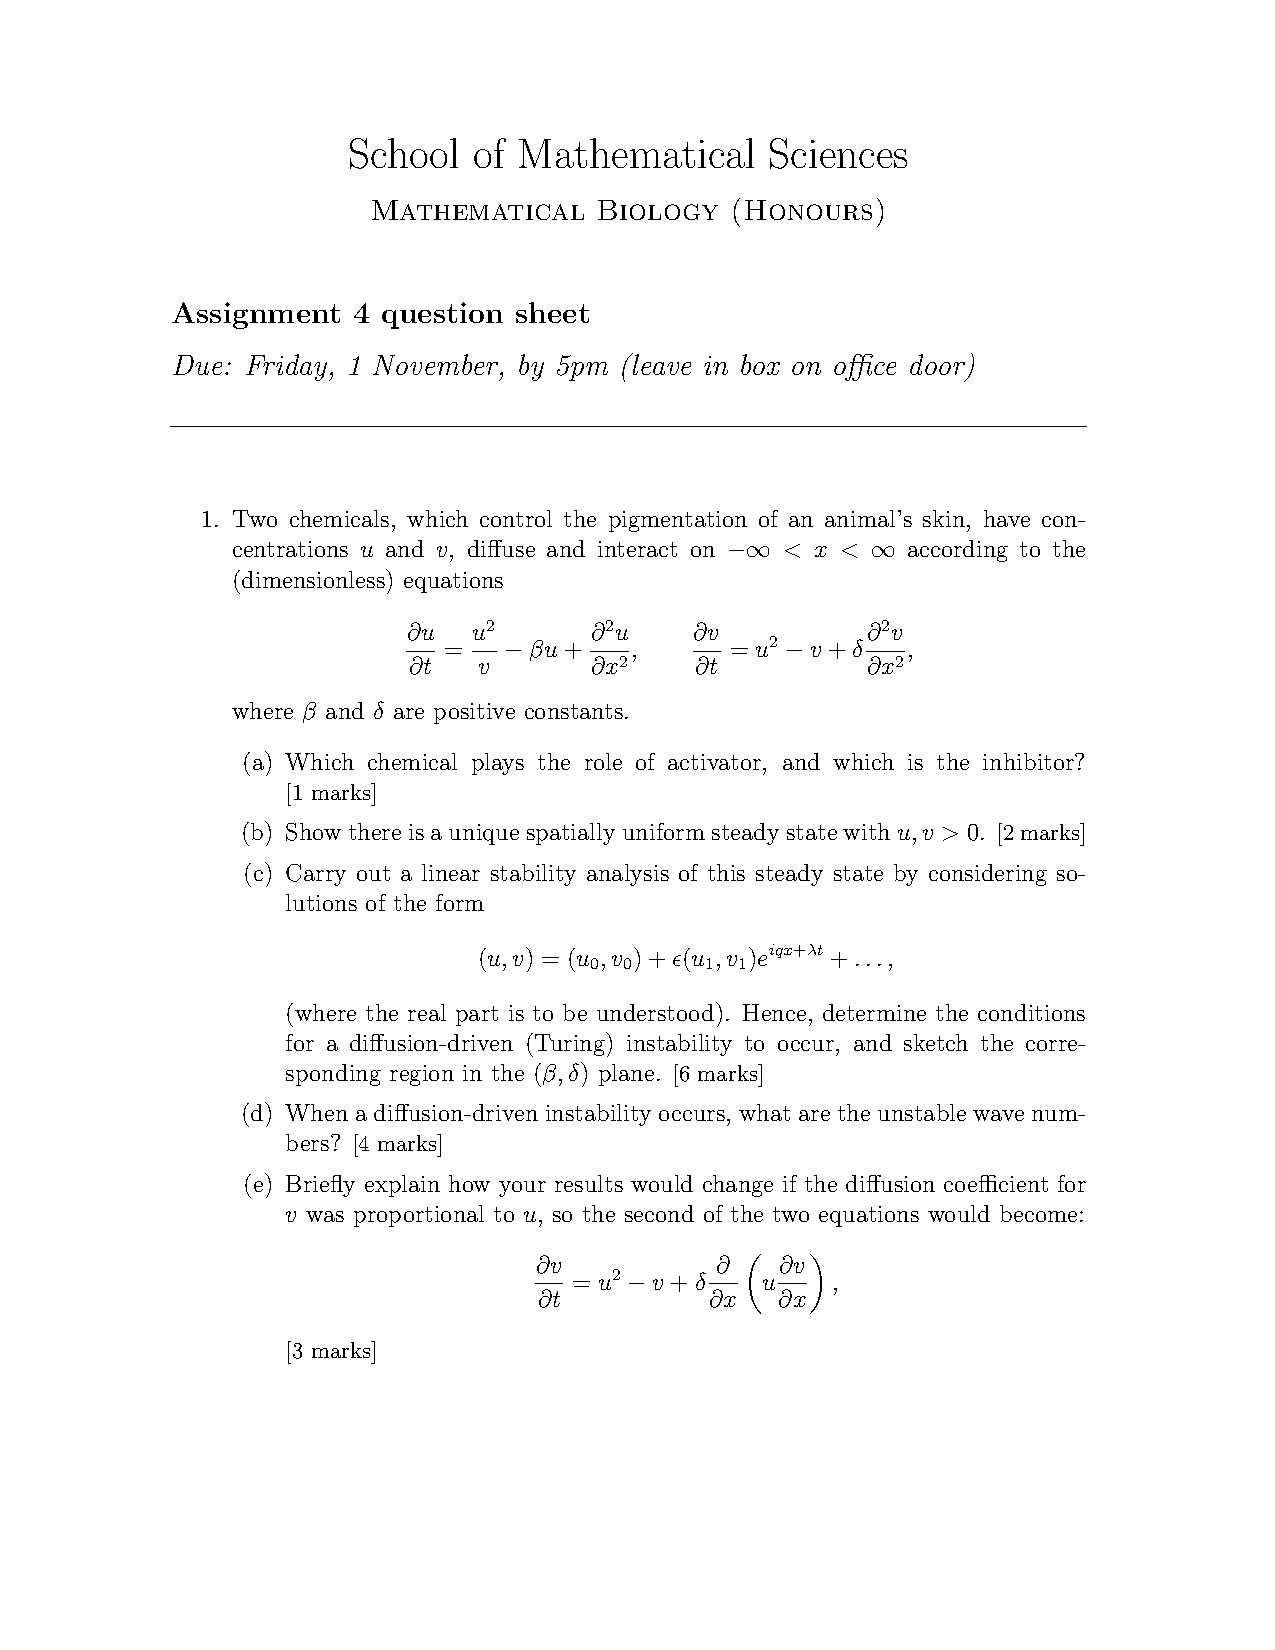
\includepdf[pages=1-]{A4_2019.pdf}


\end{document}

